\section{Semantics}
\scriptsize{Form and meaning: The Roots} \\
{\tiny Level 1: Abstract Relation\\
Level 2: Concrete Mapping (Denotation)\\
Level 3: Metalanguage (Translation)
}\\
\scriptsize{Arbitrariness} {\tiny For most words, the relation between the form (i.e. phonetic shape) of the word and its meaning is arbitrary; Onomatopoetic words are words whose forms are intended to be imitations of the sounds which they refer to. systematic non-arbitrariness, iconicity, systematicity}\\
\scriptsize{Compositionality} {\tiny two words might be productively combined to yield a new, predictable meaning. Hallmark of human language (and other communication systems) as it enables the infinite use of finite means. In the case of idioms (e.g. kicking the bucket), the intended meaning of the sentence is not a linear combinatorial derivation of its parts. Rather, a complex meaning is assigned to the whole phrase.}\\
\scriptsize{3 levels of meaning} {\tiny word meaning: sentence meaning, utterance meaning}\\
\scriptsize{Reference} {\tiny intuitively we are talking about the speaker’s use of words to “point to” something in the world}\\
\scriptsize{Semiotic Triangle(Triangle of Reference/Meaning)} {\tiny Symbol(language) - World(referent) - Thought/Reference(meaning)}\\
\scriptsize{Denotational Semantics} {\tiny focuses on the link between linguistic expressions and the world}\\
\scriptsize{Cognitive Semantics} {\tiny focuses on the link between linguistic expressions and mental representations}\\
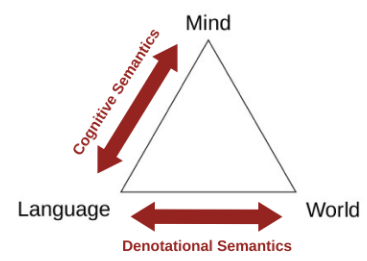
\includegraphics[scale=0.15]{triangle.png}\\
\scriptsize{Referring Expressions}\\ {\tiny Proper names (Mao Zedong)/rigid designators\\
“Natural kind” terms (the octopus, humans, methane): names of species or substances\\
Deictic elements (indexicals: you, here, now): words which refer to something in the speech situation itself.\\
Anaphoric elements (George... he..., every boy(non-referring anaphora))\\
Definite descriptions (this book, the sixteenth president): normally used in contexts where the hearer is able to identify a unique referent, but can also be used generically without referring to any specific individual \\
Indefinite descriptions (a cowboy): may be used to refer to a specific individual or may be non-specific, referring/non-referring/ambiguous
}\\
\scriptsize{Sense/Denotation}\\ {\tiny Sense: the aspects of meaning which do not depend on the context of use\\
Denotation: the sort of meaning which does depend on the context
}\\
\scriptsize{Word meaning}\\ {\tiny problem of variable reference, i.e. ambiguity, indeterminacy, vagueness\\
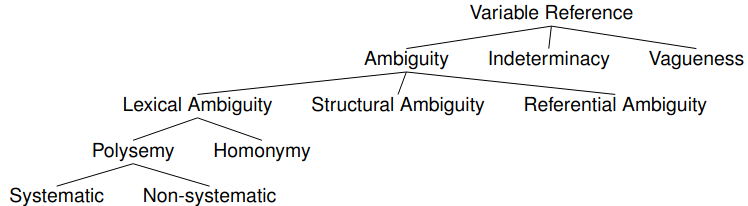
\includegraphics[scale=0.15]{variable-reference.png}\\
lexical ambiguity [ambiguous, polysemous] (e.g. beat): words that have two or more senses\\
structural ambiguity (e.g. Two cars were reported stolen by the Groveton police yesterday): the two senses arise because the grammar of the language can assign two different structures to the same string of words, even though none of those words is itself ambiguous\\
referential ambiguity: usage of anaphoric expressions with ambiguous antecendents
}\\
\scriptsize{Lexical Ambiguity}\\ {\tiny polysemy: one word with multiple senses (e.g. beat) (criteria: semantic feature/component sharing, figurative extension, existence of a primary sense, etymology)\\
homonymy: different words that happen to sound the same (e.g. can)\\
another perspective: allows for greater ease of processing by permitting efficient linguistic units to be re-used; a functional property of language that allows for greater communicative efficiency
}\\
\scriptsize{Indeterminacy} {\tiny a word can have variability in its reference despite having a single defined sense (e.g. cousin) 
}\\
\scriptsize{Vagueness} {\tiny limits of its possible denotations cannot be precisely defined (e.g. tall)
}\\
\scriptsize{Indeterminacy vs. Vagueness}\\ {\tiny context-dependence: denotation of a vague word depends on the context\\
borderline cases: vague words display borderline cases due to their gradability\\
"little-by-little" paradoxes: due to the gradability of vague words, it is hard (impossible?) to determine when a certain denotation is justified (e.g. when exactly does a person with hair become a bald person?)\\
indeterminacy tends to be language-specific, the degree to which these properties are preserved in translation
}\\
\scriptsize{Tests}\\ {\tiny Zeugma Test: on his fishing trip he caught three trout and a cold (lexically ambiguous)\\
Identity Test: John saw her duck, and so did Bill (lexically ambiguous: interpretations have to be identical)\\
Sense Relations Test: light - dark, heavy (different sets of synonyms, antonyms)\\
Contradiction Test: They are not children any more, but they are still my children (true, ambiguous)
}
\subsection*{Propositional Logic}
Why formal logic? {\tiny overcome ambiguity, determine relationships between meanings of sentences, determine meanings of setences, model compositionality, recursive system.}\\
\textbf{Definition}
Proposition {\tiny The meaning of a simple declarative sentence. The proposition expressed by a sentence is the set of possible cases [situations] of which that sentence is true.} \\
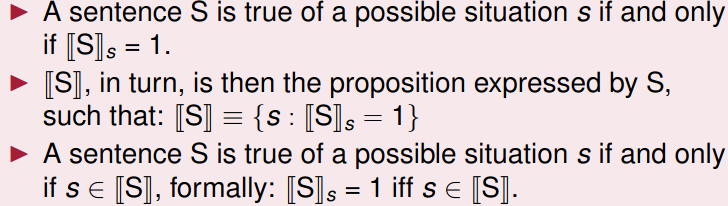
\includegraphics[scale=0.15]{proposition.png}\\
Extensions {\tiny real-world situations they refer to} \\
Frege’s Generalization {\tiny The extension of a sentence S is its truth value} \\
Types of Sentences and Propositions {\tiny Analytic sentence(tautology): true in every situation; Contradiction: false in every situation; Synthetic sentence: either true or false depending on the situation}\\
Inference {\tiny premisses: the facts which form the basis of the inference; conclusions: the fact which is inferred}\\
Syllogism {\tiny an important variety of deductive argument in which a conclusion follows from two or more premises}\\
Categorical Syllogism {\tiny A logical argument consisting of exactly three categorical propositions, two premises and the conclusion}\\
Types of Inference {\tiny inferences based on content words; logical words(propositional logic); quantifiers(predicate logic)}
\subsection*{Predicate Logic}
{\tiny Introduce constants and variables representing invididuals and predicates to capture the main structural building blocks of sentences. Introduce quantifiers to allow for quantified statements.}
\textbf{Definition}
{\tiny constant symbols: a, b, c\\
variable symbols: x, y, z\\
n-ary/n-place predicate symbols: A, B, C, reflect relations between n elements (n>0)\\
function symbols: lower case letters (f, g, etc.), take n variables (with n>=0) as their arguments, e.g. f(x): father of x\\
connectives:$\neg, \land, \lor, \to, ...$ \\
quantifiers: $\forall, \exists$ \\
round brackets (), equal sign =}\\
Universal instantiation {\tiny By using a variable x bound by the universal quantifier (Premise 1), and then specifiyng this variable as a constant symbol (Premise 2)}\\
Existential Generalization {\tiny By asserting that two predicates are true for the same constant symbol (premise 1 and premise 2)}\\
Evaluation: Model theory {\tiny a model: (i) the domain, i.e. the set of all individual entities in the situation, (ii) the denotation sets for the basic vocabulary items\\
N-place predicates are evaluated by whether the constant symbol(s) is a member of the denotation set of the predicate\\
Logical operators are evaluated the same way as in propositional logic\\
Quantifiers are evaluated according to subset relations
}\\
Valency in Semantics\\
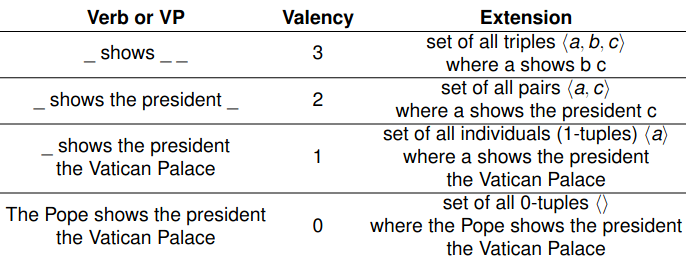
\includegraphics[scale=0.15]{valency.png}\\
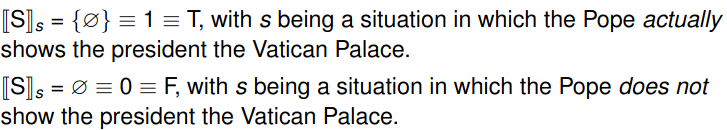
\includegraphics[scale=0.15]{0-valence.png}\\
Formal Composition {\tiny Compositional semantic theories assume that syntax and semantics work in parallel. For each phrase structure rule that combines two expressions into a larger phrase, there is a corresponding semantic rule which combines the meanings of the parts into the meaning of the newly formed expression}\\
Type theory {\tiny a formal semantic account enabling compositionality from the most basic entities (type e) to sentences (type t) in a recursive manner\\
Syntactic trees (here PSG trees) can then be mapped onto type-theoretic trees
}\\
Functional Application {\tiny If $\alpha$ is of type <b, a> and $\beta$ of type b, then $\alpha(\beta)$ is of type a}\\
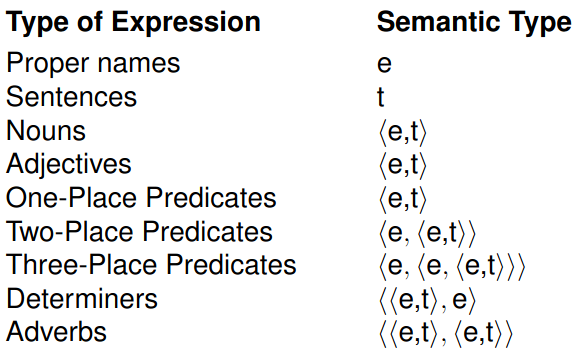
\includegraphics[scale=0.15]{types.png}\\
